	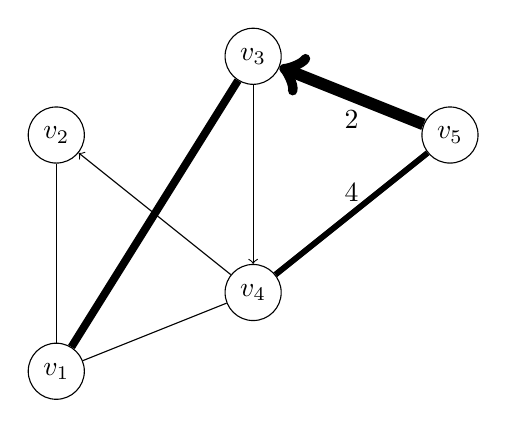
\begin{tikzpicture}
		% cette commande permet de créer un noeud, en précisant sa position spatiale (les valeurs entre parenthèses) et le texte qu'il contient (entre accolades). 
        %On peut également donner un nom interne au noeud (ici : A, B, C, D, etc.), qui sera utilisé plus tard par Tikz lors de la création des liens.
        \node[shape=circle,draw=black] (nnnn) at (0,0) {$v_1$};
		\node[shape=circle,draw=black] (node) at (0,3) {$v_2$};
		\node[shape=circle,draw=black] (truc) at (2.5,4) {$v_3$};
		\node[shape=circle,draw=black] (D) at (2.5,1) {$v_4$};
		\node[shape=circle,draw=black] (Zz) at (5,3) {$v_5$} ;
        
    	% cette commande ajoute un lien entre les noeuds dont les noms sont indiqués entre parenthèses
		\draw (nnnn) -- (node);
        \draw (nnnn) -- (D);
        % on peut changer l'épaisseur des liens de la façon suivante (pour les graphes pondérés)
		\draw[line width=1mm] (nnnn)  -- (truc);
        % toujours pour les graphes pondérés, on peut aussi rajouter des labels sur les liens (les positions optionnelles possibles sont left/right et above/below)
		\draw[line width=0.75mm] (D) -- (Zz) node [midway, left, above] {4};
		% on peut aussi orienter les liens de la façon suivante
        \draw[->] (truc) -- (D);
        % pour changer la taille de la flèche
        \draw[-{>[scale=1.5]}] (D) -- (node);
        % et on peut bien sûr combiner tout ça
        \draw[-{>[scale=2]}, line width=1.5mm] (Zz) -- (truc) node [midway, left, below] {2};
	% fin du diagramme
	\end{tikzpicture}
